\documentclass[11pt]{article}
\usepackage[top=0.9in,bottom=0.9in,left=1.0in,right=1.0in]{geometry}
\usepackage{amsmath,amssymb,amsthm}
\usepackage{graphicx}
\usepackage{booktabs}
\usepackage{enumitem}
\usepackage{xcolor}
\usepackage[colorlinks=true,linkcolor=blue!55!black,urlcolor=blue!55!black]{hyperref}
\usepackage{parskip}
\usepackage{titlesec}
\usepackage{caption}
\captionsetup{font=small}
\titlespacing*{\section}{0pt}{12pt}{5pt}
\titlespacing*{\subsection}{0pt}{9pt}{3pt}

\theoremstyle{remark}
\newtheorem*{observation}{Observation}

\newcommand{\Sw}{S_W}
\newcommand{\Sb}{S_B}
\newcommand{\St}{S_T}
\newcommand{\rank}{\operatorname{rank}}

\title{\vspace{-1.3cm}\textbf{Eigenfaces vs.\ Fisherfaces}\\[3pt]
\large Implementation, experiments and results\\[2pt]
\normalsize CS 740 course project}
\date{}

\begin{document}
\maketitle
\vspace{-1.1cm}

{\small
\setlength{\parskip}{0pt}
\tableofcontents
}

\vspace{4pt}\hrule\vspace{10pt}

%======================================================================
\section{What we did}

We implement Belhumeur, Hespanha \& Kriegman, \emph{``Eigenfaces vs.\
Fisherfaces: Recognition Using Class Specific Linear Projection''}, IEEE TPAMI
19(7), 1997, and then run seven experiments of our own on top of it.

The paper's argument is short. PCA keeps the directions of largest
\emph{variance}. Under changing illumination the largest variance is the
lighting, not the identity, so PCA preserves exactly the wrong thing. Fisher's
linear discriminant instead keeps the directions that best separate the
\emph{classes}, which discounts the variation PCA holds on to.

\subsection{The experiments}

\begin{center}
\small
\begin{tabular}{llp{7.0cm}}
\toprule
 & data & question \\
\midrule
Toy  & synthetic 2-D & Can we \emph{see} PCA choosing the wrong direction? \\
Main & ORL, Yale     & Four methods compared head to head. \\
\midrule
E1 & ORL, Yale & How badly conditioned is $\Sw$ as $m$ grows, and is the
                  paper's $m=N-c$ actually the best choice? \\
E2 & ORL       & Is the result real, or is the pipeline leaking labels? \\
E3 & ORL       & Can we choose $m$ \emph{without} looking at the test set? \\
E4 & ORL       & Fisherfaces are higher-frequency. Does that make them more
                  fragile under noise, as the theory predicts? \\
E5 & Yale      & How does error grow with the angle of the light source? \\
E6 & ORL       & Does the $c-1$ ceiling on the number of Fisherfaces really
                  bind? \\
E7 & ORL       & A different question entirely: is this person wearing
                  glasses? \\
\bottomrule
\end{tabular}
\end{center}

E1--E4 and E6 are ours. E5 is modelled on the paper's Section 3.1 protocol and
E7 follows its Section 3.3.

\subsection{Relation to the paper}

\textbf{Implemented:} the Fisherfaces algorithm in full, and three of the
paper's four methods --- correlation, eigenfaces (including the ``drop the
first three components'' variant) and Fisherfaces.

\textbf{Not implemented:} the \emph{Linear Subspace} method of Section 2.3,
which builds a separate 3-D illumination subspace for each person.

\textbf{Different data.} The paper's lighting experiment uses the Harvard
database, which comes from a 1995 PhD thesis and has no surviving public
download; its expression experiment uses a 1997 Yale set that is smaller and
different from the one distributed today. We used instead:

\begin{center}
\small
\begin{tabular}{llll}
\toprule
database & size & what varies & role here \\
\midrule
ORL        & $40\times10$, $92\!\times\!112$    & pose, expression, glasses & the hard case for LDA \\
CroppedYale & $38\times\!\sim\!64$, $168\!\times\!192$ & illumination only  & the paper's claim \\
\bottomrule
\end{tabular}
\end{center}

CroppedYale is by the same authors (2001) and is the modern successor to the
Harvard set, with 38 subjects rather than 5. E5 is therefore \emph{modelled on}
the paper's protocol rather than a reproduction of it.

%======================================================================
\section{Theory}

Only the mathematics the code actually uses. Full derivations are in the
accompanying study guide.

\subsection{Notation}

\begin{center}
\small
\begin{tabular}{cll}
\toprule
symbol & meaning & value here \\
\midrule
$d$        & pixels per image               & ORL $10304$, Yale $32256$ \\
$N$        & training images                & ORL $192$, Yale $1520$ \\
$c$        & people (classes)               & ORL $32$, Yale $38$ \\
$n_j$      & training images of person $j$  & ORL $6$, Yale $40$ \\
$m$        & PCA dimension kept before LDA  & swept in E1 \\
$x$        & one image as a column          & $x\in\mathbb{R}^d$ \\
$\bar{x}$  & the mean face                  & \\
$X$        & centred training images as columns & $d\times N$ \\
$U$        & the eigenfaces, as columns     & \\
$W$        & the Fisherfaces, as columns    & $d\times(c-1)$ \\
$\Sw,\Sb,\St$ & within-, between- and total-class scatter & \\
\bottomrule
\end{tabular}
\end{center}

Each image is unrolled column-by-column into a vector (\texttt{im(:)} in
MATLAB). This discards the knowledge that neighbouring pixels are adjacent,
which is legitimate because every image is unrolled the same way, so
corresponding pixels land in corresponding coordinates.

\subsection{Eigenfaces and the \texorpdfstring{$L = X^{\!\top}\!X$}{L = X'X} trick}

PCA needs the top eigenvectors of the covariance $C = \tfrac1N XX^{\!\top}$,
which is $d\times d$. For Yale that is $32256^2$, about $8.3$\,GB, so we cannot
even store it. We do not have to. Let $L = X^{\!\top}\!X$, which is only
$N\times N$. If $Lw = \lambda w$, multiply on the left by $X$:
\[
  X\big(X^{\!\top}\!Xw\big) = X(\lambda w)
  \qquad\Longrightarrow\qquad
  \big(XX^{\!\top}\big)(Xw) = \lambda\,(Xw),
\]
so $Xw$ is an eigenvector of $XX^{\!\top}$ with the \emph{same} eigenvalue. We
solve a $192\times192$ problem instead of a $10304\times10304$ one.

The same calculation gives
$\|Xw\|^2 = w^{\!\top}X^{\!\top}\!Xw = \lambda$, so $\|Xw\| = \sqrt{\lambda}$
and \emph{not} $1$. The columns must therefore be renormalised, or the
projection stops being orthogonal.

\subsection{Fisher's criterion}

With class means $\mu_j$ and overall mean $\bar{x}$,
\[
  \Sw=\sum_{j=1}^{c}\sum_{x\in X_j}(x-\mu_j)(x-\mu_j)^{\!\top},
  \qquad
  \Sb=\sum_{j=1}^{c}n_j(\mu_j-\bar{x})(\mu_j-\bar{x})^{\!\top},
\]
and we maximise
\[
  J(w)=\frac{w^{\!\top}\Sb\,w}{w^{\!\top}\Sw\,w},
\]
whose stationary points satisfy the \emph{generalised} eigenproblem
$\Sb w=\lambda\Sw w$. Note that $J$ is unchanged when $w$ is scaled, because
numerator and denominator are both quadratic --- a fact that matters in
Section~\ref{sec:unitnorm}.

\subsection{Two rank bounds that decide everything}

\textbf{$\rank(\Sb)\le c-1$.} $\Sb$ is a sum of $c$ rank-one terms spanned by
the vectors $\mu_j-\bar{x}$, and those obey one linear relation:
$\sum_j n_j(\mu_j-\bar{x}) = N\bar{x}-N\bar{x} = 0$. A set of $c$ vectors with
a dependence spans at most $c-1$ dimensions. \textbf{So there are at most $c-1$
Fisherfaces, however many pixels or images we have.}

\textbf{$\rank(\Sw)\le N-c$.} Within class $j$ the $n_j$ centred columns sum to
zero, so they span at most $n_j-1$ dimensions. Summing,
$\sum_j(n_j-1)=N-c$. Read this as \emph{degrees of freedom}: each person
donates only $n_j-1$ directions to $\Sw$. ORL donates \textbf{5} per person,
Yale \textbf{39}.

\textbf{Why the two-stage algorithm exists.} In pixel space $\Sw$ is $d\times d$
with rank at most $N-c$ ($1482 \ll 32256$ on Yale), so it is singular, $\Sw^{-1}$
does not exist and $J$ is undefined. The fix is to project onto $m$ PCA
directions first. Combining the bounds, $m$ is squeezed from both sides:
\[
  \boxed{\;c-1 \;\le\; m \;\le\; N-c\;}
\]
the lower bound because $c-1$ directions cannot be extracted from a space of
fewer than $c-1$ dimensions. We found that one by crashing the E1 sweep.

\subsection{Solving the generalised eigenproblem}

$\Sw^{-1}\Sb$ is not symmetric --- its transpose is $\Sb\Sw^{-1}$ --- so the
textbook route is to use the Cholesky factorisation $\Sw=R^{\!\top}R$ and
substitute $w=R^{-1}z$:
\[
  \Sb R^{-1}z=\lambda R^{\!\top}RR^{-1}z=\lambda R^{\!\top}z
  \quad\xrightarrow{\ \times R^{-\top}\ }\quad
  \underbrace{R^{-\top}\Sb R^{-1}}_{M}z=\lambda z ,
\]
and $M^{\!\top}=R^{-\top}\Sb^{\!\top}R^{-1}=M$, so a generalised problem has
become an ordinary \emph{symmetric} one: real eigenvalues, orthogonal
eigenvectors. The paper specifies none of this --- it says only ``the
generalized eigenvectors of $\Sb$ and $\Sw$'' --- so the solver is our choice.
In the code we call \texttt{eig(Sb,Sw)}, having measured that it and explicit
Cholesky whitening agree to $0.00^\circ$.

\subsection{The step that is easy to miss}
\label{sec:unitnorm}

\texttt{eig(Sb,Sw)} returns columns satisfying $W^{\!\top}\Sw W = I$. They are
$\Sw$-orthogonal, \textbf{not} Euclidean-orthogonal, so their ordinary lengths
differ by orders of magnitude --- a factor of $287$ on ORL. $J$ does not care,
because it is scale-invariant. But our classifier is nearest neighbour with
\emph{Euclidean} distance, which is \emph{not} scale-invariant: a coordinate
whose basis vector is long contributes more to every distance, so a few
directions dominate every comparison.

\begin{observation}
Normalising each Fisherface to unit length is therefore not cosmetic. Without
it Fisherfaces score $\mathbf{29.5\%}$ on ORL; with it, $\mathbf{90.6\%}$. The
subspace, the eigenvalues and the theory are identical in both cases --- only
the basis lengths differ. This was a real bug in our first implementation.
\end{observation}

%======================================================================
\section{Results}

ORL uses 6 training and 4 test images for each of 32 people; Yale uses 40
training images for each of 38. Classification is nearest neighbour in the
projected space throughout.

\subsection{The toy problem}

Two 2-D classes sharing a covariance $\Sigma=\mathrm{diag}(16,\,0.25)$, with
means differing only in $y$. All the \emph{spread} is along $x$ and all the
\emph{class information} is along $y$ --- a trap built for PCA.

\begin{figure}[htbp]
\centering
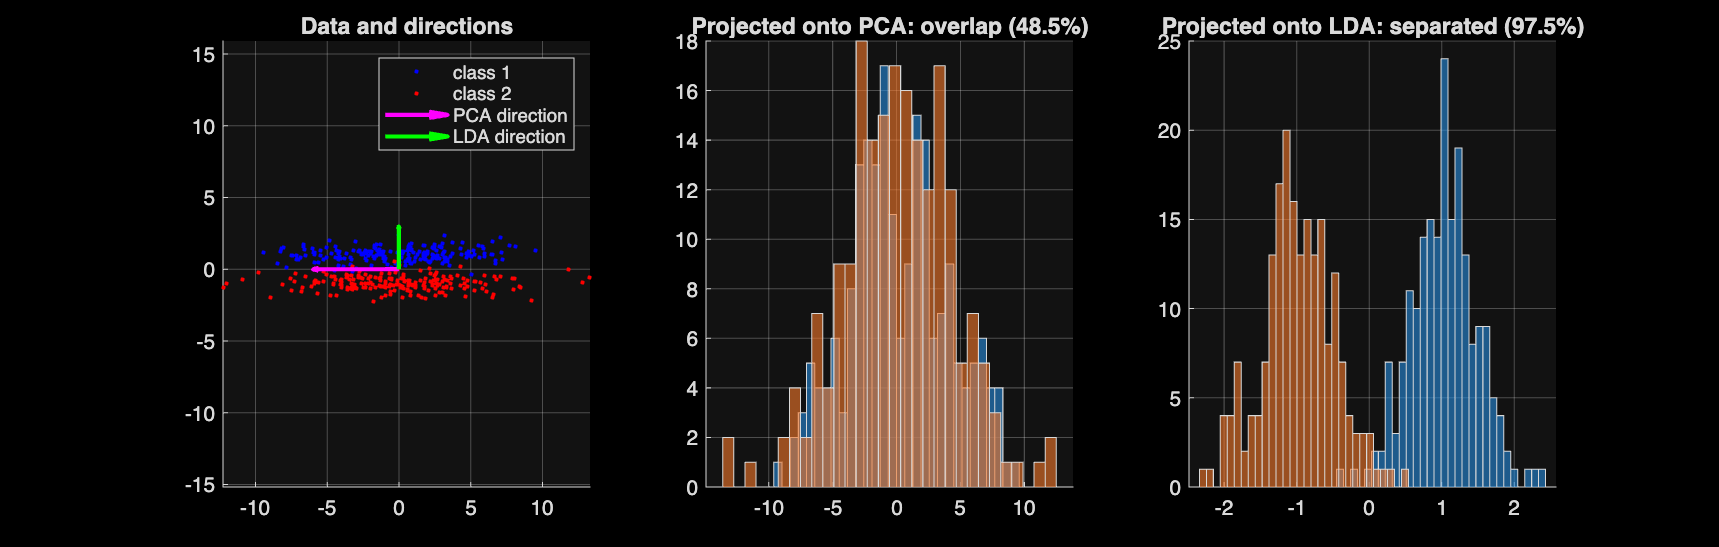
\includegraphics[width=\textwidth]{figures/toy.png}
\caption{PCA picks the $x$-axis, the direction of greatest variance, and the
two classes become inseparable ($48.5\%$ error, chance being $50\%$). Fisher
picks the $y$-axis and separates them almost perfectly ($97.5\%$ accuracy).
The whole argument of the paper, in two dimensions.}
\end{figure}

\subsection{The main comparison}

\begin{center}
\small
\begin{tabular}{lcccc}
\toprule
 & correlation & eigenfaces (best $k$) & eigenfaces ($k=c-1$) & \textbf{Fisherfaces} \\
\midrule
ORL  & 91.4\% & \textbf{95.3\%} & 94.5\% & 90.6\% \\
Yale & 43.0\% & 34.2\% & 29.5\% & \textbf{67.2\%} \\
\bottomrule
\end{tabular}
\end{center}

The $k=c-1$ column exists so that eigenfaces and Fisherfaces are compared with
the \emph{same number of features}; otherwise the comparison is unfair.

\textbf{On Yale the paper's claim reproduces clearly}: Fisherfaces roughly
double eigenfaces. Two further checks agree with the paper --- dropping the top
three principal components raises Yale from $34.2\%$ to $58.7\%$, because they
encode lighting, and the same operation \emph{hurts} ORL
($95.3\%\to87.5\%$), where they encode identity.

\textbf{On ORL Fisherfaces lose}, to eigenfaces at matched dimension ($90.6$
against $94.5$) and even to raw-pixel correlation ($91.4$). We report this
rather than tune it away. The mechanism is an asymmetry in how the two methods
use their matrices: eigenfaces never estimates $\Sw$ and keeps the
\emph{largest} eigenvalues of a well-estimated $\St$, whereas Fisherfaces must
\emph{invert} $\Sw$ and so leans on its \emph{smallest} eigenvalues, which are
the worst estimated --- and ORL supplies only 5 degrees of freedom per person.

\begin{figure}[htbp]
\centering
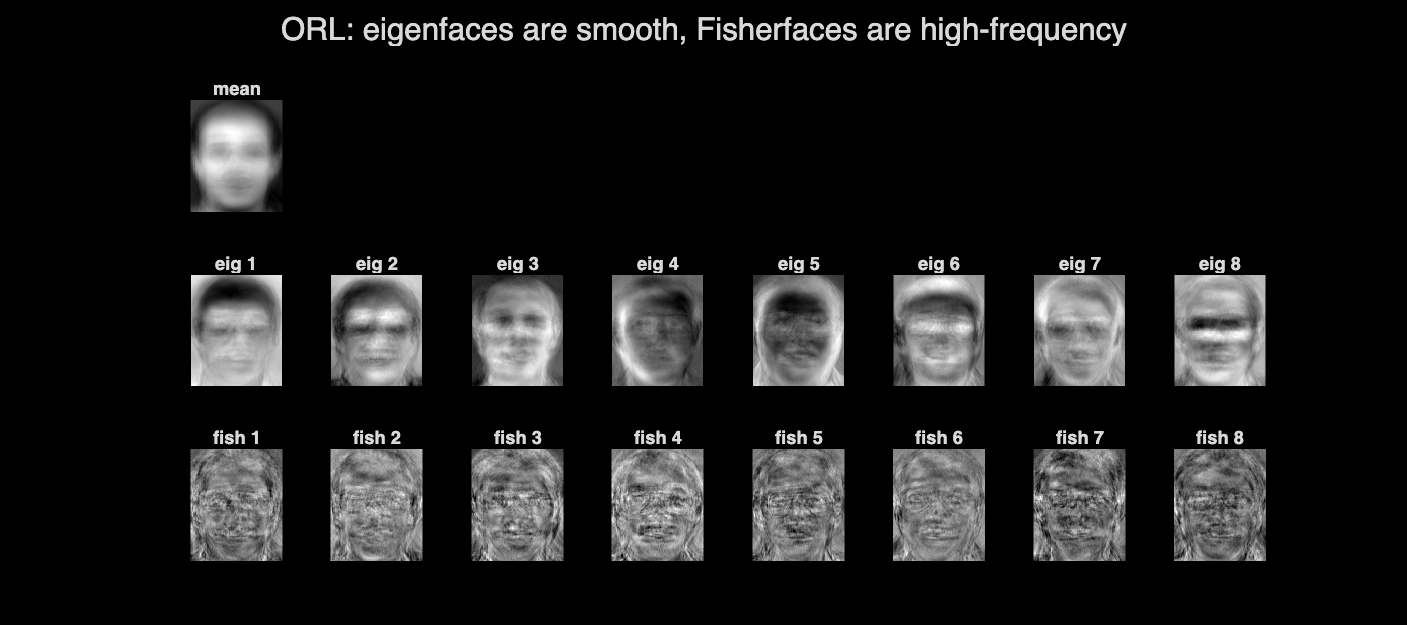
\includegraphics[width=0.495\textwidth]{figures/ORL_faces.png}
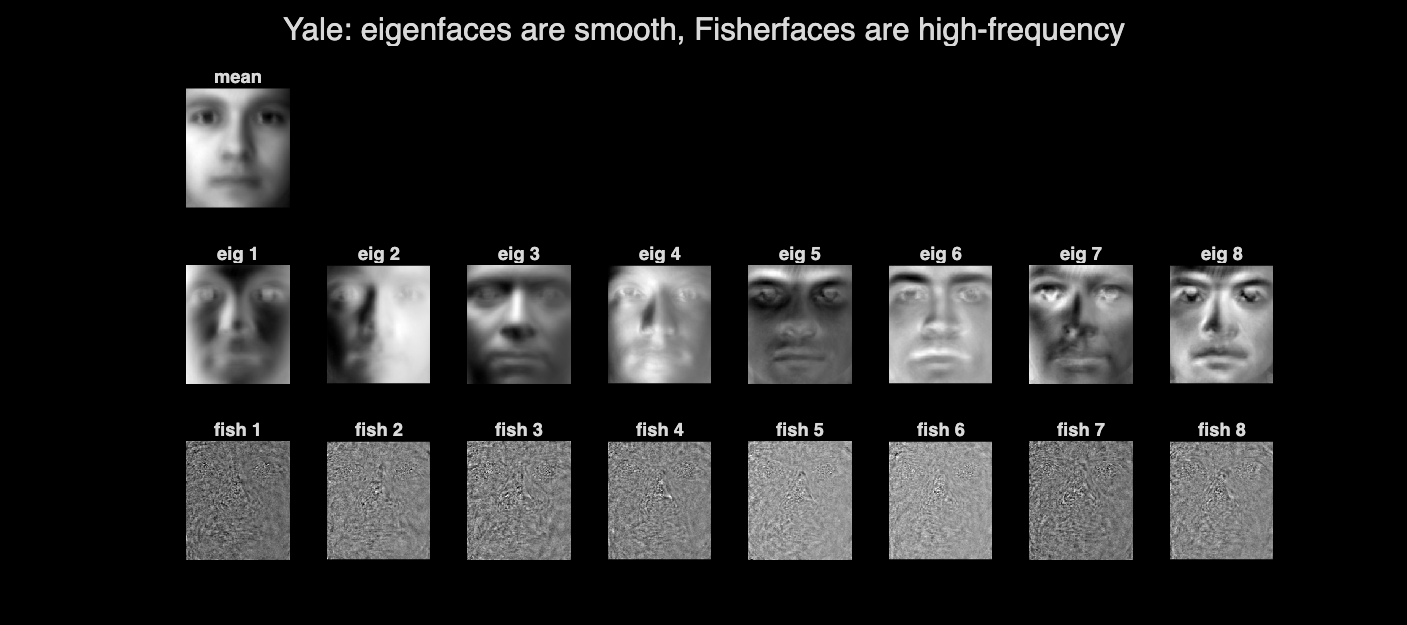
\includegraphics[width=0.495\textwidth]{figures/Yale_faces.png}
\caption{Mean face, top eigenfaces and top Fisherfaces, for ORL (left) and
Yale (right). Eigenfaces are smooth and face-like; Fisherfaces are
high-frequency and concentrate around the eyes and brow. This is predicted,
not incidental: whitening scales direction $l$ by $1/\sqrt{\lambda_l}$ and so
amplifies the low-variance, fine-detail directions most.}
\end{figure}

\clearpage

\subsection{E1: sweeping the PCA dimension \texorpdfstring{$m$}{m}}

The paper fixes $m=N-c$. At that value $\Sw$ has rank $m$: full rank, but with
\emph{zero slack} --- one more direction and it would be singular. We swept $m$
and recorded both the accuracy and $\kappa(\Sw)$, the ratio of largest to
smallest eigenvalue, which says how much relative error gets amplified.

\begin{figure}[htbp]
\centering
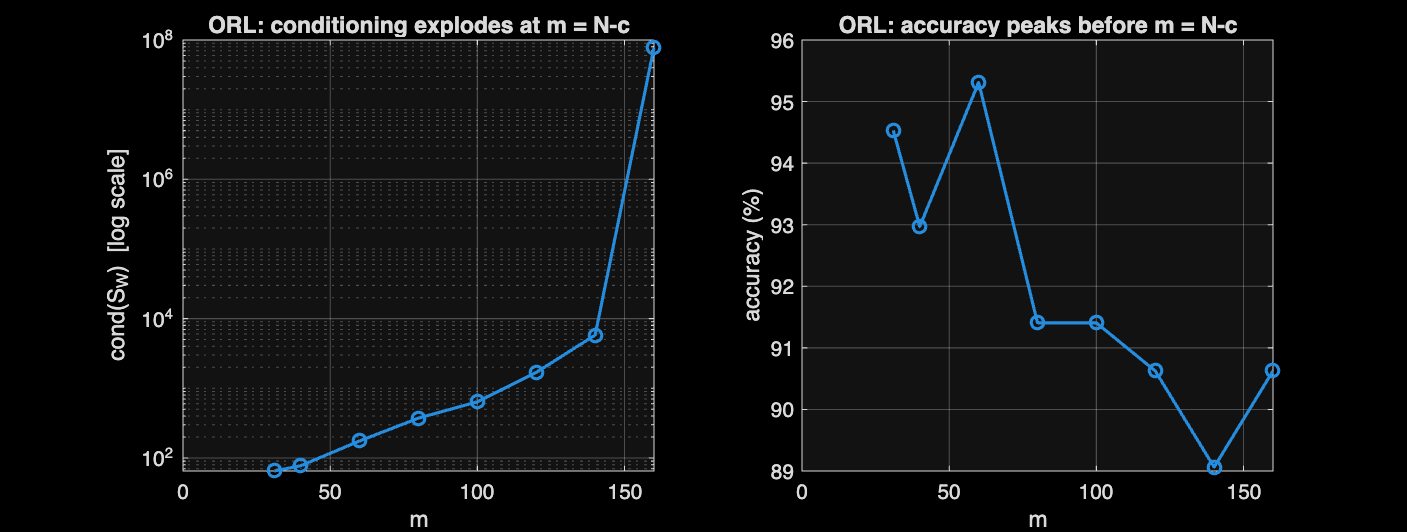
\includegraphics[width=0.95\textwidth]{figures/E1_sweep_m_ORL.png}\\[3pt]
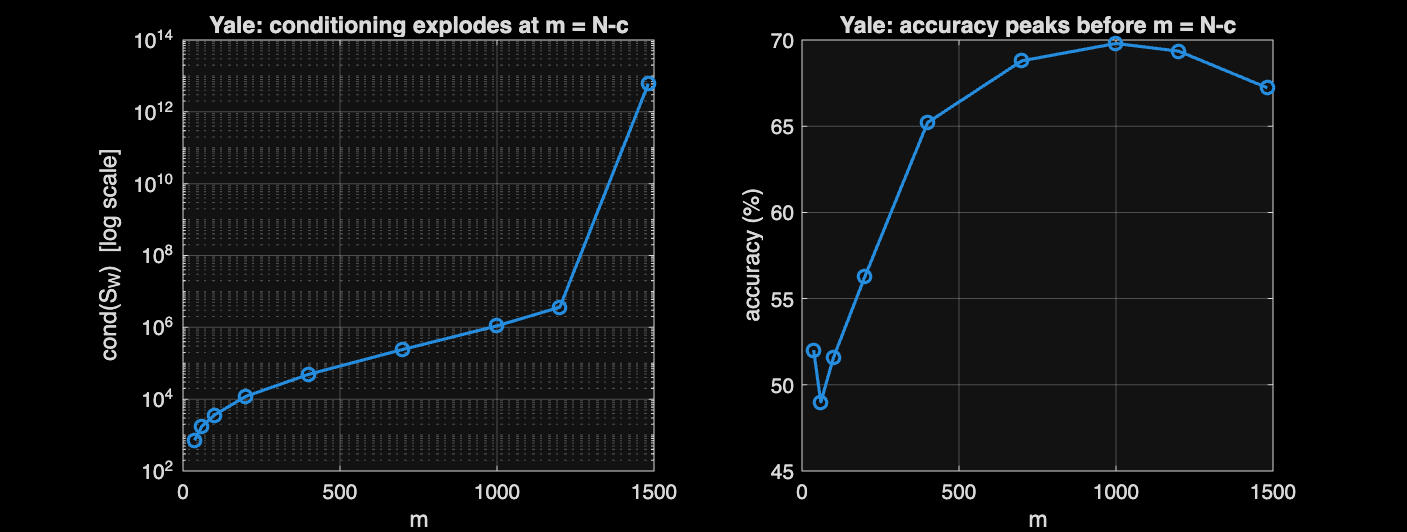
\includegraphics[width=0.95\textwidth]{figures/E1_sweep_m_Yale.png}
\caption{Conditioning (log scale) and accuracy against $m$, for ORL (top) and
Yale (bottom). Conditioning is flat for most of the range and then turns
almost vertical in the last few steps, while accuracy has already peaked and
started falling.}
\end{figure}

\begin{center}
\small
\begin{tabular}{rrr@{\hskip 2.5em}rrr}
\toprule
\multicolumn{3}{c}{\textbf{ORL} ($N-c = 160$)} & \multicolumn{3}{c}{\textbf{Yale} ($N-c = 1482$)} \\
$m$ & rate & $\kappa(\Sw)$ & $m$ & rate & $\kappa(\Sw)$ \\
\midrule
 31 & 94.5\% & $6.5\times10^{1}$ &  100 & 51.6\% & $3.6\times10^{3}$ \\
 60 & \textbf{95.3\%} & $1.8\times10^{2}$ &  400 & 65.2\% & $4.9\times10^{4}$ \\
120 & 90.6\% & $1.7\times10^{3}$ & 1000 & \textbf{69.8\%} & $1.1\times10^{6}$ \\
140 & 89.1\% & $5.8\times10^{3}$ & 1200 & 69.4\% & $3.6\times10^{6}$ \\
160 & 90.6\% & $\mathbf{7.9\times10^{7}}$ & 1482 & 67.2\% & $\mathbf{6.0\times10^{12}}$ \\
\bottomrule
\end{tabular}
\end{center}

\begin{observation}
\textbf{The paper's $m=N-c$ is not the best choice on either database.} ORL
peaks at $m=60$ with $95.3\%$ against $90.6\%$ at $m=160$; Yale peaks at
$m=1000$ with $69.8\%$ against $67.2\%$ at $m=1482$. Accuracy turns down well
before conditioning becomes alarming, so this is not purely a numerical
effect --- the extra directions are fitting noise.
\end{observation}

\paragraph{Is the peak predictable?} Partly. There is no closed form, because
it is a bias--variance trade-off that depends on the data. But the controlling
quantity is not $m$, it is the sampling ratio $\gamma = m/(N-c)$. The
Marchenko--Pastur law says a covariance estimated in $m$ dimensions from that
many samples has condition number roughly
$\big((1+\sqrt{\gamma})/(1-\sqrt{\gamma})\big)^{2}$, which \emph{diverges as
$\gamma\to1$} --- and $\gamma=1$ is exactly $m=N-c$. Comparing that prediction
with our ORL measurements, the ratio between them is $9.8$, $10.1$, $8.8$ and
$6.5$ at $m=31,60,100,140$: nearly constant, because the measured conditioning
factorises into the intrinsic conditioning of the true $\Sw$ (about $9$) times
the sampling inflation. The blow-up near $m=N-c$ is a sampling artefact, and a
predictable one.

\subsection{E2: is the result real?}

Shuffle the training labels and change nothing else. Now no face has any
relation to its label, so nothing should beat guessing at $100/c = 3.1\%$.

\begin{figure}[htbp]
\centering
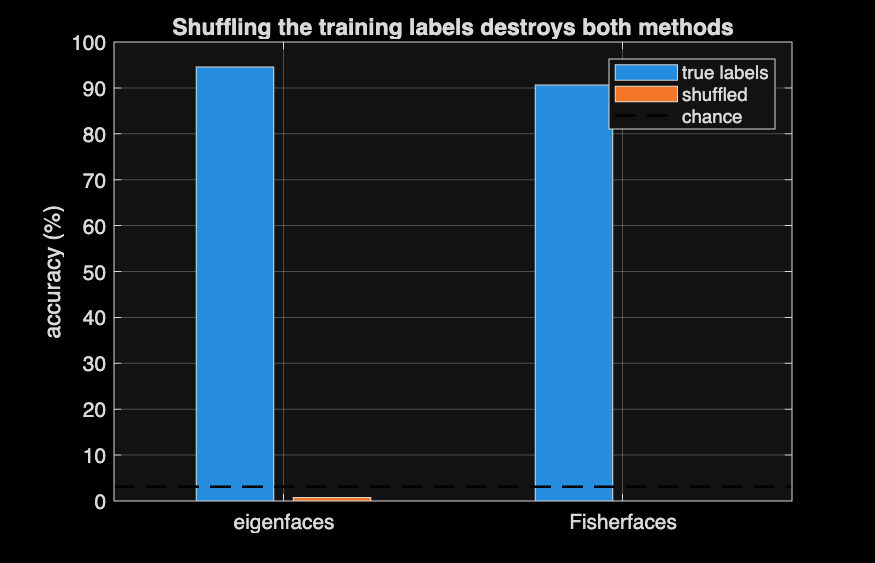
\includegraphics[width=0.56\textwidth]{figures/E2_label_permutation.png}
\caption{Eigenfaces fall from $94.5\%$ to $0.8\%$ and Fisherfaces from
$90.6\%$ to $0.0\%$. The headline numbers are not an artefact of the pipeline.}
\end{figure}

\begin{observation}
Both land \emph{below} chance rather than at it, and that is not a fluke. The
shuffle is applied to training labels only, so Fisherfaces faithfully learns to
separate the \emph{shuffled} grouping; a test face is then projected near the
training images that genuinely look like it, and those now carry somebody
else's label by construction. The method is systematically wrong, not randomly
wrong.
\end{observation}

\subsection{E3: choosing \texorpdfstring{$m$}{m} without looking at the test set}

E1 read ``the best $m$'' off the test column. That is tuning on the test set,
and a number obtained that way is optimistic. The honest procedure is
cross-validation \emph{inside} the training set: six-fold leave-one-out, with
the PCA basis recomputed per fold so the validation image cannot leak into it.

\begin{figure}[htbp]
\centering
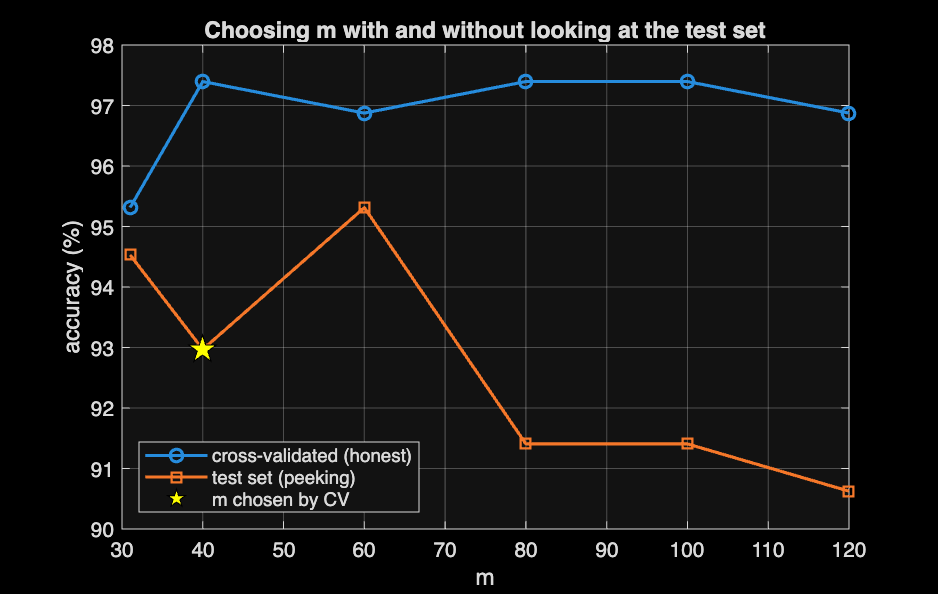
\includegraphics[width=0.58\textwidth]{figures/E3_cross_validation.png}
\caption{The honest curve and the peeking curve. The star marks the $m$ that
cross-validation selects, evaluated once on the test set.}
\end{figure}

\begin{observation}
Cross-validation picks $m=40$, scoring $\mathbf{93.0\%}$. Tuning on the test
set would have picked $m=60$ for $95.3\%$. \textbf{The $2.3$-point gap is the
optimism avoided by not peeking}, and $93.0\%$ is our honest estimate. Note
also that the cross-validated rates sit \emph{above} the test rates: the
validation images come from the same six-image pool as the training images,
which is an easier problem. Cross-validation is used here to \emph{rank}
values of $m$, not to estimate the final accuracy.
\end{observation}

\subsection{E4: a prediction, tested}

Fisherfaces are higher-frequency than eigenfaces, because whitening amplifies
the low-variance fine-detail directions. White pixel noise has energy at every
frequency. \textbf{Prediction: Fisherfaces should degrade faster.} This is the
only experiment here that could have failed.

\begin{figure}[htbp]
\centering
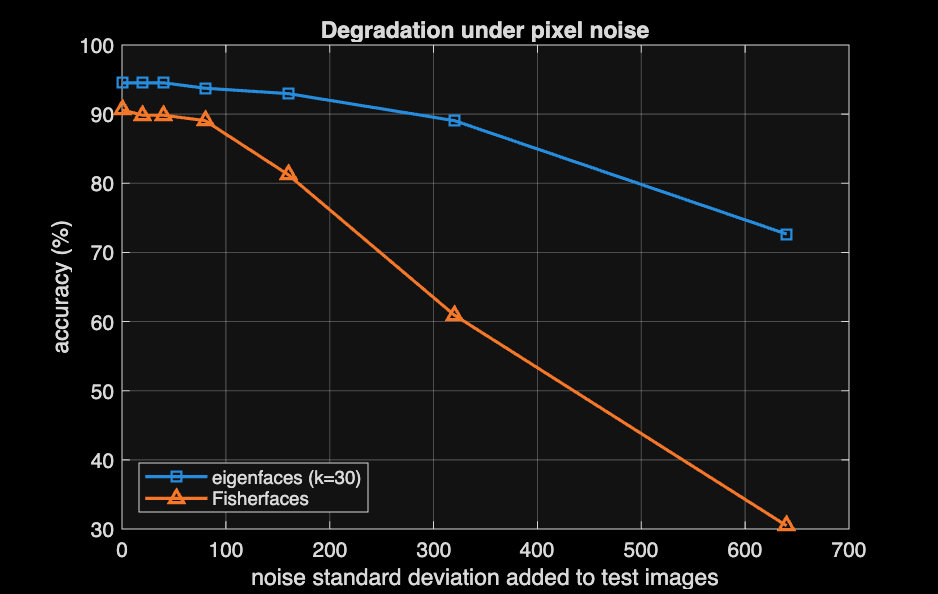
\includegraphics[width=0.58\textwidth]{figures/E4_noise.png}
\caption{Accuracy against the standard deviation of noise added to the test
images. The curves are flat until $\sigma\approx160$ and then separate sharply.}
\end{figure}

\begin{observation}
Confirmed, with a caveat worth stating. From $\sigma=0$ to $640$, Fisherfaces
lose $\mathbf{60.2}$ points against eigenfaces' $\mathbf{21.9}$ --- roughly
three times more fragile. But \textbf{the effect only appears far beyond
realistic noise.} Our first attempt stopped at $\sigma=80$ and found nothing:
all methods moved $0.8$ points, which on 128 test images is exactly
\emph{one image}. Projection is a strong denoiser, so $\sigma$ must become
very large before anything happens at all.
\end{observation}

\subsection{E5: error against lighting angle}

The paper does not report one Yale number; it bins the test images by how far
the light is from the camera axis. Every Yale filename encodes the direction,
e.g.\ \texttt{yaleB01\_P00A+020E-40.pgm} means azimuth $+20^\circ$, elevation
$-40^\circ$, and the angle from the optical axis is
$\theta=\arccos(\cos\text{az}\cdot\cos\text{el})$.

\begin{figure}[htbp]
\centering
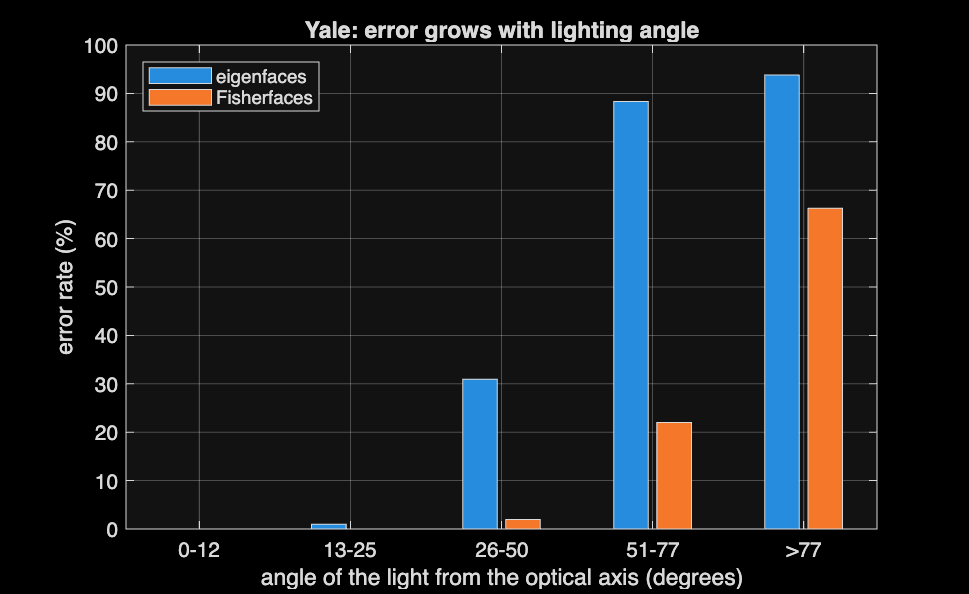
\includegraphics[width=0.62\textwidth]{figures/E5_lighting_angle.png}
\caption{Error against lighting angle. The first bin is drawn as a gap, not a
zero bar, because it contains no test images at all.}
\end{figure}

\begin{center}
\small
\begin{tabular}{lccccc}
\toprule
angle & $0$--$12^\circ$ & $13$--$25^\circ$ & $26$--$50^\circ$ & $51$--$77^\circ$ & $>77^\circ$ \\
images & 0 & 104 & 152 & 300 & 338 \\
\midrule
eigenfaces  & --- & 1.0\% & 30.9\% & 88.3\% & 93.8\% \\
Fisherfaces & --- & \textbf{0.0\%} & \textbf{2.0\%} & \textbf{22.0\%} & \textbf{66.3\%} \\
\bottomrule
\end{tabular}
\end{center}

\begin{observation}
Error climbs with angle for both methods and the gap \emph{widens}: at
$26$--$50^\circ$ Fisherfaces are $15\times$ better, and even in the hardest bin
they halve the error. This is the paper's central claim measured where it
actually bites, rather than averaged into one aggregate number.
\end{observation}

\begin{observation}[The empty first bin is itself a finding]
There are \textbf{no} test images at $0$--$12^\circ$, and this is not a parsing
bug. Lighting is encoded as \texttt{A+020}/\texttt{A-020}, and \texttt{dir}
sorts names as text where \texttt{'+'} precedes \texttt{'-'}. Taking the first
40 files per subject therefore puts all the near-frontal lighting into
training. Every test image is at least $12^\circ$ off axis and $638$ of the
$894$ are beyond $50^\circ$ --- the test set is not a random sample of lighting
conditions, it is the hard tail of one. That is why the headline Yale figures
look so poor; randomising the split roughly doubles every method.
\end{observation}

\subsection{E6: sweeping the number of classes}

$\rank(\Sb)\le c-1$, so there are at most $c-1$ Fisherfaces. We varied $c$ to
see whether that ceiling really binds.

\begin{figure}[htbp]
\centering
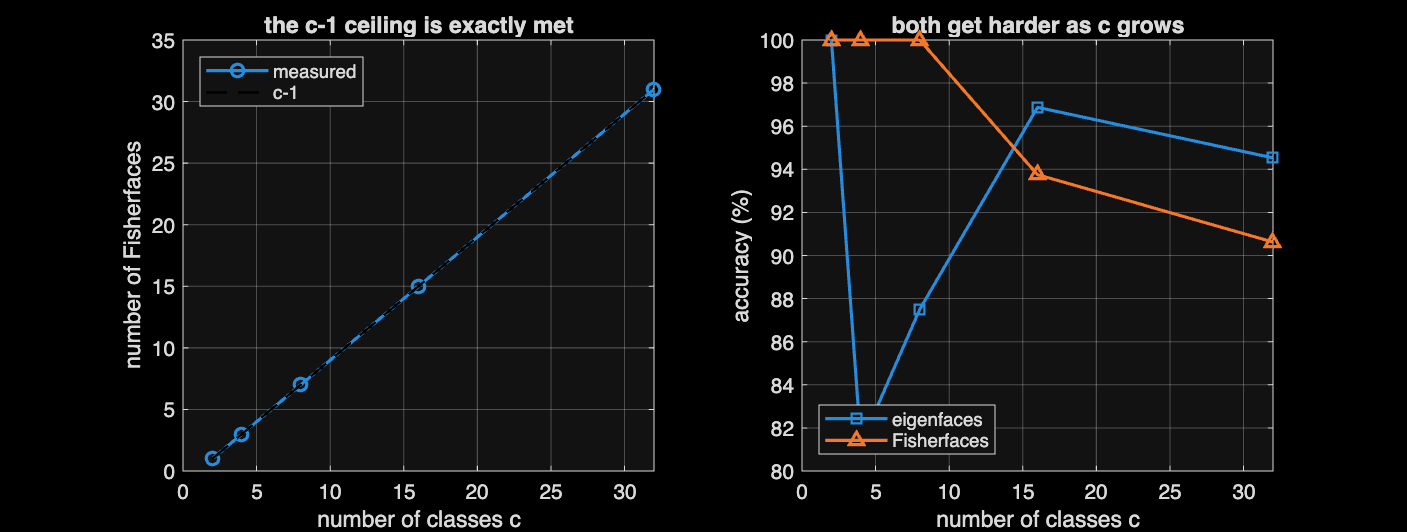
\includegraphics[width=0.95\textwidth]{figures/E6_number_of_classes.png}
\caption{Left: the number of Fisherfaces produced, against $c-1$. Right:
accuracy as the problem grows.}
\end{figure}

\begin{center}
\small
\begin{tabular}{rrrrr}
\toprule
$c$ & 2 & 4 & 8 & 16 \\
\midrule
Fisherfaces produced & 1 & 3 & 7 & 15 \\
eigenfaces  & 100.0\% & 81.2\% & 87.5\% & 96.9\% \\
Fisherfaces & 100.0\% & 100.0\% & 100.0\% & 93.8\% \\
\bottomrule
\end{tabular}
\end{center}

\begin{observation}
The number of Fisherfaces equals $c-1$ on every row, so the rank bound is a
live constraint and not merely a proof on a page. Fisherfaces reach $100\%$ for
$c\le8$ and fall to $90.6\%$ at $c=32$ as the problem gets harder.
\end{observation}

\subsection{E7: glasses or no glasses}

A different question: not \emph{who} is this, but \emph{is this person wearing
glasses}. With $c=2$, $\rank(\Sb)\le1$ and there is exactly \textbf{one}
Fisherface --- the whole decision rests on a single direction.

ORL ships no glasses labels, so we labelled all 400 images by inspection: 117
wear glasses and 8 people appear both with and without, which is what makes the
question non-trivial. We balanced the set $50/50$ --- otherwise always
answering ``no'' scores $70.8\%$ and beats every method --- and used
leave-one-\emph{subject}-out, so the test face is never seen in training and
the classifier cannot cheat by recognising the person.

\begin{figure}[htbp]
\centering
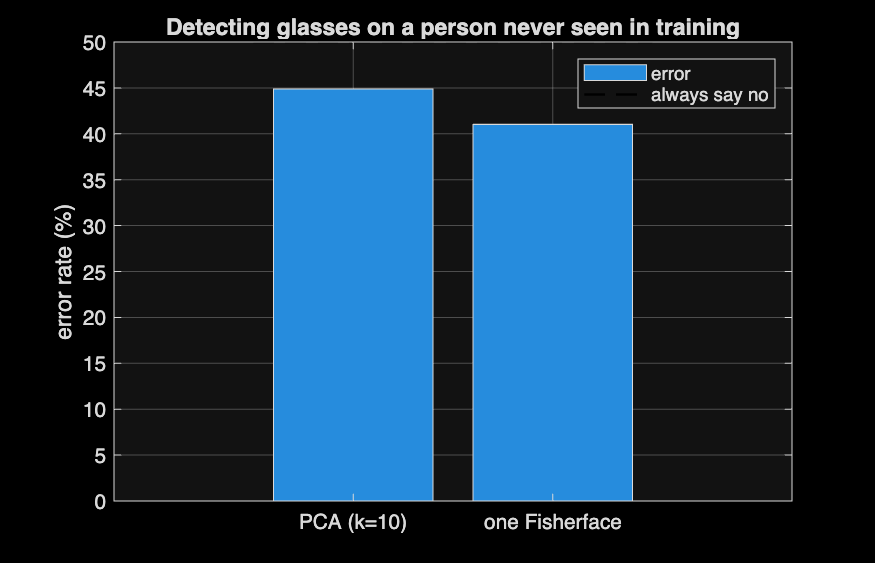
\includegraphics[width=0.52\textwidth]{figures/E7_glasses.png}
\caption{Error rate on a person never seen during training. The dashed line is
the $50\%$ a coin would achieve on this balanced set.}
\end{figure}

\begin{center}
\small
\begin{tabular}{lcc}
\toprule
method & our error & the paper's error \\
\midrule
PCA, $k=10$          & 44.9\%          & 52.6\% \\
one Fisherface       & \textbf{41.0\%} & \textbf{5.3\%} \\
always answer ``no'' & 50.0\%          & 50.0\% \\
\bottomrule
\end{tabular}
\end{center}

\begin{observation}
\textbf{We reproduce the paper's finding that PCA is near chance, but not that
Fisherfaces solve the task.} We believe the difference is the data rather than
the method: the paper's 36 images were \emph{paired} --- the same person
photographed with and without glasses in one session, same lighting --- so
glasses were the only thing that changed. In ORL glasses co-vary with pose,
expression and session, so the single Fisher direction has no clean signal to
lock onto. This is a negative result and we report it as one.
\end{observation}

%======================================================================
\section{Conclusions}

\begin{enumerate}[leftmargin=1.4em,itemsep=3pt]

\item \textbf{The paper's claim holds, and it is mechanistic.} When
within-class variation is large, structured and shared across people ---
illumination on Yale --- discounting it is worth far more than the cost of
estimating it, and Fisherfaces win decisively ($67.2\%$ against $34.2\%$, and
$15\times$ lower error in the mid-angle bin). When it is small and
idiosyncratic --- pose and expression on ORL --- the estimation cost dominates
and plain PCA, or even no projection at all, does better.

\item \textbf{Degrees of freedom alone do not explain it.} It is tempting to
blame ORL's five degrees of freedom per person, but E6 shows Fisherfaces at
$100\%$ for $c\le8$ on the \emph{same} six-images-per-person data, and E5 shows
them $15\times$ better than eigenfaces in Yale's mid-angle bin. What decides
the outcome is how much \emph{structured} within-class variation there is to
remove --- large, shared and nearly low-dimensional on Yale; small and
idiosyncratic on ORL.

\item \textbf{$m=N-c$ is defensible but not optimal.} Better accuracy at
smaller $m$ on both databases, with $\kappa(\Sw)$ five orders of magnitude
smaller there. The blow-up at $\gamma=m/(N-c)\to1$ is predicted by
Marchenko--Pastur, so this is not a quirk of our data.

\item \textbf{Our honest accuracy on ORL is $93.0\%$, not $95.3\%$.} The
difference is whether $m$ was chosen by cross-validation or by looking at the
test set.

\item \textbf{The results are real.} Destroying the training labels destroys
the performance, which is the check that makes everything above worth quoting.

\item \textbf{Two things that look like failures and are not:} Fisherfaces at
$29.5\%$ on ORL was a missing unit-norm step, not a failure of LDA; and the
empty $0$--$12^\circ$ lighting bin is a filename-sorting accident in the split,
not a parsing bug. Both cost us time, and both are the kind of thing that is
invisible until the numbers are questioned.
\end{enumerate}

%======================================================================
\section*{Code, data and reproducing this}
\addcontentsline{toc}{section}{Code, data and reproducing this}

Three scripts, each with its helper functions at the bottom:

\begin{center}\small
\begin{tabular}{ll}
\toprule
file & what it runs \\
\midrule
\texttt{toy.m}                       & the 2-D toy problem \\
\texttt{eigenfaces\_vs\_fisherfaces.m} & the main comparison, ORL and Yale \\
\texttt{experiments.m}               & experiments E1--E7 \\
\bottomrule
\end{tabular}
\end{center}

\noindent They need base MATLAB only, and write every figure in this report
into \texttt{figures/}. Each number quoted above appears in the
\texttt{run\_log} files.

Code: \href{https://github.com/qascade/eigenfaces-vs-fisherfaces}{\texttt{github.com/qascade/eigenfaces-vs-fisherfaces}}.
The databases are not redistributed there, because Extended Yale B's terms
forbid incorporating its images into a larger publicly distributed database
without permission. Download them from
\href{https://www.cl.cam.ac.uk/research/dtg/attarchive/facedatabase.html}{Cambridge}
(ORL) and
\href{https://datarepo.eng.ucsd.edu/visiondata/iskwak/public_html/ExtYaleDatabase/ExtYaleB.html}{UCSD}
(Extended Yale B, cropped), unzip both one level above the code, and run
\texttt{./rename\_yale.sh} once --- the Yale folders ship as
\texttt{yaleB01}--\texttt{yaleB39} with \texttt{yaleB14} absent, which is not a
countable range. Renaming changes no result, because the class label is the
loop index and never the folder name.

\end{document}
